\chapter{圖片與表格}\label{cha:figures}

準備好章節內容後，就可以開始加入圖片與表格。本章會先示範單張圖片，再說明並排圖片、網格圖片、傳統表格與三線表的寫法。初次使用時，建議先將範例貼進自己的章節，確認能正常編譯，再替換圖片路徑、標題與數據。

模板會自動產生編號，預設將圖片與表格的標題都放在下方；需要更換位置時，可以依\ref{sec:caption}的說明調整。以下圖片與數字都是排版範例，換成論文內容時，請一併修改標題和說明。

\section{插入單張圖片}

若要插入圖片，建議將圖片放進 \code{figures/} 資料夾中，再將檔案路徑填入 \code{\fig}。以下使用專案附帶的 \code{figures/samples/architecture.png}，路徑從專案根目錄算起。方括號裡的 \code{0.6\linewidth} 則將圖片寬度設為目前可用排版寬度的六成，可以先照範例編譯，再依圖片內容調整大小；省略方括號時，寬度預設為 \code{0.8\linewidth}。

\begin{lstlisting}[language=latex]
\fig[0.6\linewidth]{figures/samples/architecture.png}{研究架構}{fig:one}
\end{lstlisting}

編譯結果如\figref{fig:one}所示，使用預設設定時，圖片下方會顯示自動產生的編號與標題中的文字。三個大括號依序是圖片路徑、標題與標籤；替換圖片時，請一起修改路徑與標題。若是複製範例來新增另一張圖，也要更換最後的 \code{fig:one} 標籤，讓每張圖都有不同的名稱，供內文引用；不需要引用的話，可以留成 \code{{}}。

\fig[0.6\linewidth]{figures/samples/architecture.png}{研究架構}{fig:one}

如果需要自行設定圖片的其他選項，第一個方括號可以直接寫成 \code{\includegraphics} 認得的寬度，較複雜的情形則不用 \code{\fig}，改用標準的 \code{figure} 寫法，再自己呼叫 \code{\includegraphics}：

\begin{lstlisting}[language=latex]
\begin{figure}[htbp]
  \centering
  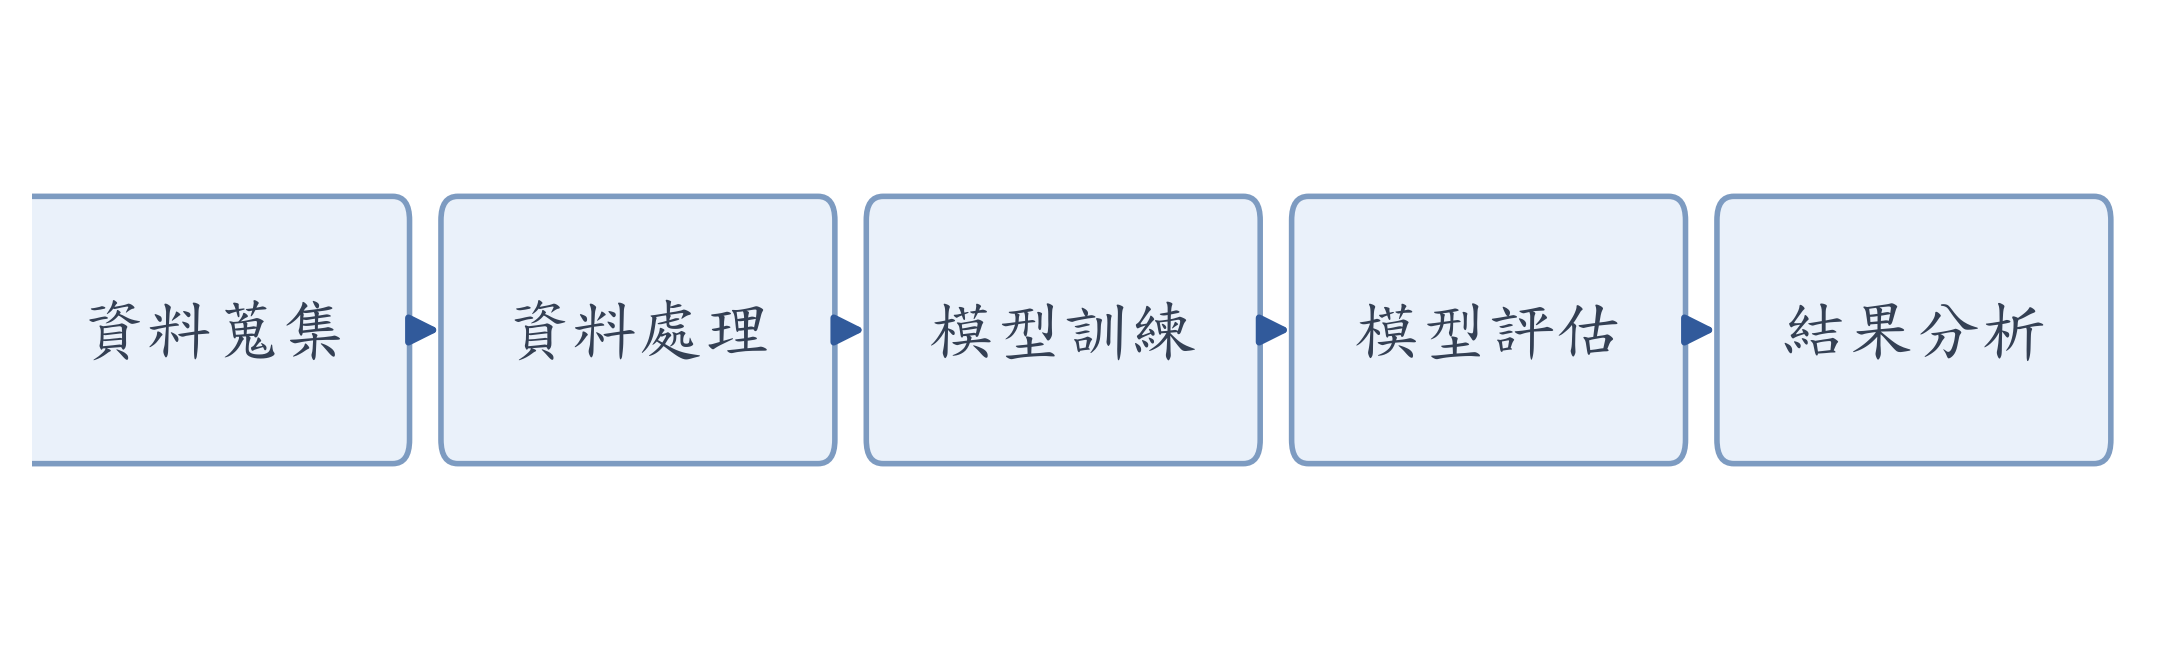
\includegraphics[width=0.6\linewidth,height=5cm,keepaspectratio]{figures/samples/architecture.png}
  \caption{說明}
  \label{fig:custom}
\end{figure}
\end{lstlisting}

\code{width} 設定圖片顯示寬度；\code{0.6\linewidth} 是目前可用排版寬度的六成，也可以寫成 \code{8cm} 等固定長度。\code{height} 設定顯示高度，不指定時會依原圖比例自動計算。同時給寬與高時，圖片會被拉伸變形，除非再加上 \code{keepaspectratio}，此時圖片保留完整與原比例，縮放到不超出這個區域。

其他常用選項有 \code{page}（插入多頁 PDF 的第幾頁，預設 \code{1}）、\code{trim} 與 \code{clip}（裁切圖片邊緣）。完整參數可參考 \href{https://ctan.org/pkg/graphicx}{graphicx 的文件}。這種標準寫法的圖片不會照著 \code{layout.caption-position.image} 調整標題位置，標題要放在上方就把 \code{\caption} 寫在 \code{\includegraphics} 之前。

\section{並排圖片}

要將兩張圖片放在同一列時，可以使用 \code{figrow} 環境，依序填入各張圖片的路徑與小標題。小標題會自動加上 \code{(a)}、\code{(b)} 等編號，整組圖片則共用一個圖號與總標題，在圖次中也只會列出一筆。以下示範兩張圖片的寫法：

\begin{lstlisting}[language=latex]
\begin{figrow}{函數圖形比較}{fig:row}
  \subfig{figures/samples/sin-x.pdf}{$\sin x$}
  \subfig{figures/samples/x-sin-x.pdf}{$x \sin x$}
\end{figrow}
\end{lstlisting}

\begin{figrow}{函數圖形比較}{fig:row}
  \subfig{figures/samples/sin-x.pdf}{$\sin x$}
  \subfig{figures/samples/x-sin-x.pdf}{$x \sin x$}
\end{figrow}

若不需要小標題，第二個大括號留空即可。編譯後若覺得圖片靠得太近，可以在環境後面加上 \code{[gutter=2em]}，增加兩欄之間的距離，再觀察圖片是否仍有足夠的顯示空間。

\begin{lstlisting}[language=latex]
\begin{figrow}[gutter=2em]{函數圖形比較}{}
  \subfig{figures/samples/sin-x.pdf}{}
  \subfig{figures/samples/x-sin-x.pdf}{}
\end{figrow}
\end{lstlisting}

此外，並排圖片的 \code{width} 是相對於各自那一欄的寬度，例如 \code{[width=0.8]} 時，每張圖會占自己欄寬的八成。需要縮小圖片時可以從這個數值調整，不必先修改原始圖檔。

\section{網格圖片}

如果圖片較多，希望分成數列排列，可以改用 \code{figgrid}。\code{rows} 指定列數，\code{columns} 指定每列的欄數。下面放入四張圖片，設定 \code{rows=2}、\code{columns=2}，就會由左到右、由上而下排成兩列。每張圖的小標題與整組圖片的總標題，寫法都和並排圖片相同。

\begin{lstlisting}[language=latex]
\begin{figgrid}[rows=2,columns=2,placement=auto]{模型預測結果}{fig:grid}
  \subfig{figures/samples/a.pdf}{線性模型}
  \subfig{figures/samples/b.pdf}{決策樹}
  \subfig{figures/samples/c.pdf}{隨機森林}
  \subfig{figures/samples/d.pdf}{神經網路}
\end{figgrid}
\end{lstlisting}

\begin{figgrid}[rows=2,columns=2,placement=auto]{模型預測結果}{fig:grid}
  \subfig{figures/samples/a.pdf}{線性模型}
  \subfig{figures/samples/b.pdf}{決策樹}
  \subfig{figures/samples/c.pdf}{隨機森林}
  \subfig{figures/samples/d.pdf}{神經網路}
\end{figgrid}

四張圖使用相同的合成訓練資料：空心圓點是觀測值，黑色實線是各模型的預測結果。這些數據只用於示範排版，並非真實論文的實驗結果。\code{placement=auto} 讓 \LaTeX{} 把圖組當成一般浮動體，依剩餘版面決定留在原位或移到合適的位置；省略時為 \code{placement=none}，圖組會固定在寫下的位置。\code{figrow} 與 \code{\fig} 也可以加上同一個選項，例如 \code{\fig[width=0.6\linewidth,placement=auto]\{...\}}。

若要排成兩列、每列三張，可設定 \code{rows=2,columns=3}。圖片會依照填入的順序重新排列；下例在前四張模型圖後加入 k 近鄰與支援向量迴歸，剛好填滿六格。\code{rows} 可以省略，讓列數隨圖片數量自動增加；若指定列數，圖片數量不可超過 \code{rows * columns}。調整後請確認圖片中的文字仍能清楚閱讀；若縮得太小，可以減少每列的欄數。

\begin{lstlisting}[language=latex]
\begin{figgrid}[rows=2,columns=3]{兩列三欄排版示例}{fig:grid-2x3}
  \subfig{figures/samples/a.pdf}{線性模型}
  \subfig{figures/samples/b.pdf}{決策樹}
  \subfig{figures/samples/c.pdf}{隨機森林}
  \subfig{figures/samples/d.pdf}{神經網路}
  \subfig{figures/samples/e.pdf}{k 近鄰}
  \subfig{figures/samples/f.pdf}{支援向量迴歸}
\end{figgrid}
\end{lstlisting}

編譯結果如\figref{fig:grid-2x3}所示：

\begin{figgrid}[rows=2,columns=3]{兩列三欄排版示例}{fig:grid-2x3}
  \subfig{figures/samples/a.pdf}{線性模型}
  \subfig{figures/samples/b.pdf}{決策樹}
  \subfig{figures/samples/c.pdf}{隨機森林}
  \subfig{figures/samples/d.pdf}{神經網路}
  \subfig{figures/samples/e.pdf}{k 近鄰}
  \subfig{figures/samples/f.pdf}{支援向量迴歸}
\end{figgrid}

\section{表格}

表格有兩種寫法：需要逐格框線時，用 \code{tbl} 環境；只要表頭上下與表尾三條線的三線表，則用模板提供的 \code{tlt} 環境。兩者的資料填法相同，差別只在外觀與框線，可以依論文或系所規定挑一種。

\subsection{傳統表格}

需要每個儲存格都有框線時，使用 \code{tbl} 環境。它的參數依序是標題、標籤與欄位格式，欄位格式跟 \code{tabular} 一樣：\code{ccc} 指定三欄置中，欄與欄之間加上 \code{|} 就會畫出直線。資料由左到右、由上而下填入，\code{&} 隔開儲存格，\code{\\} 結束一列，\code{\hline} 畫橫線。

\begin{lstlisting}[language=latex]
\begin{tbl}{實驗結果（傳統表格）}{tbl:traditional}{|c|c|c|}
  \hline
  批次大小 & 準確率（\%） & 訓練時間（秒） \\
  \hline
  32  & 91.2 & 48 \\
  64  & 92.8 & 31 \\
  128 & 92.1 & 22 \\
  \hline
\end{tbl}
\end{lstlisting}

\begin{tbl}{實驗結果（傳統表格）}{tbl:traditional}{|c|c|c|}
  \hline
  批次大小 & 準確率（\%） & 訓練時間（秒） \\
  \hline
  32  & 91.2 & 48 \\
  64  & 92.8 & 31 \\
  128 & 92.1 & 22 \\
  \hline
\end{tbl}

相鄰儲存格可以合併。\code{\multicolumn{2}{c}{文字}} 讓一格橫跨兩欄；以下三欄表格的「總計」列只填兩格，因為「100 筆」已占用後兩欄，不必再補第三格。若要讓一格縱跨兩列，可改用 \code{\multirow{2}{*}{文字}}；下一列被占用的位置留空即可。

\begin{lstlisting}[language=latex]
\begin{tbl}{合併儲存格示例}{tbl:merged}{|c|c|c|}
  \hline
  項目 & 訓練集 & 測試集 \\
  \hline
  樣本數 & 80 & 20 \\
  \hline
  總計 & \multicolumn{2}{c|}{100 筆} \\
  \hline
\end{tbl}
\end{lstlisting}

\begin{tbl}{合併儲存格示例}{tbl:merged}{|c|c|c|}
  \hline
  項目 & 訓練集 & 測試集 \\
  \hline
  樣本數 & 80 & 20 \\
  \hline
  總計 & \multicolumn{2}{c|}{100 筆} \\
  \hline
\end{tbl}

\subsection{三線表}

不同於逐格加框的傳統表格，三線表源自 \href{https://apastyle.apa.org/style-grammar-guidelines/tables-figures/tables}{APA 格式}的表格慣例，在社會科學、教育、心理學等偏重統計數據的領域最為常見。少了多條直向與橫向的格線，版面更乾淨，整欄都是數字時尤其容易閱讀。\code{docs/} 收錄的各校官方論文格式規範，大多沒有指定表格要用哪種框線，實際採用哪一種通常是系所或指導教授的學術慣例，而非學校統一規定，撰寫前建議先確認清楚。

三線表的特色是：只保留表頭上下與表尾的三條橫線。使用 \code{tlt} 時，上下兩條線由環境自動畫好，表頭下方的線則自己寫一個 \code{\midrule}。以下沿用前面的資料，方便比較。

\begin{lstlisting}[language=latex]
\begin{tlt}[notes={數值為排版示例。}]{實驗結果彙整}{tbl:batch}{ccc}
  批次大小 & 準確率（\%） & 訓練時間（秒） \\
  \midrule
  32  & 91.2 & 48 \\
  64  & 92.8 & 31 \\
  128 & 92.1 & 22 \\
\end{tlt}
\end{lstlisting}

\begin{tlt}[notes={數值為排版示例。}]{實驗結果彙整}{tbl:batch}{ccc}
  批次大小 & 準確率（\%） & 訓練時間（秒） \\
  \midrule
  32  & 91.2 & 48 \\
  64  & 92.8 & 31 \\
  128 & 92.1 & 22 \\
\end{tlt}

完成資料填寫後，可以依內容調整欄寬、對齊方式與表下說明。方括號裡的選項與後面三個參數如下：

\begin{tlt}{三線表常用參數}{tbl:tlt-args}{L{0.2\linewidth}L{0.7\linewidth}}
參數 & 用途與範例 \\
\midrule
欄位格式 & \code{l}、\code{c}、\code{r} 依內容排寬；\code{L{4cm}} 是固定寬度、靠左的欄，文字較長時使用。 \\
\code{width} & 選項。給定總寬度（例：\code{width=\linewidth}）時，欄位格式可用 \code{X} 平分剩餘寬度；儲存格內有 \code{\code} 時請改用 \code{L{...}}。 \\
\code{thick}、\code{thin} & 選項。上下線／表頭線的粗細；只改這張表就傳選項，全部表格一起改就改 \code{tw-thesis.sty} 表格區塊開頭的 \code{\heavyrulewidth}。 \\
\code{notes} & 選項。表下補充說明，字級為本文字級的九成。 \\
\code{notes-label} & 選項。註記開頭；預設「註：」，設成空的 \code{{}} 可取消。 \\
\end{tlt}

若資料較多，一頁放不下整張表格，\code{tlt} 與 \code{tbl} 不會自動跨頁，請改用 \code{longtable} 環境，並自己加上 \code{\toprule}、\code{\midrule}、\code{\bottomrule}；它的 \code{\endhead} 會讓表頭在每一頁重複出現。完成後請檢查分頁位置，確認讀者能辨認各欄的資料。

三線表也能合併儲存格：如下方範例，「總計」列雖然只填兩格，實際仍占滿三欄；與上方的傳統表格相比，差別只在框線樣式。

\begin{lstlisting}[language=latex]
\begin{tlt}{三線表合併儲存格}{tbl:tlt-merged}{ccc}
  項目 & 訓練集 & 測試集 \\
  \midrule
  樣本數 & 80 & 20 \\
  總計 & \multicolumn{2}{c}{100 筆} \\
\end{tlt}
\end{lstlisting}

\begin{tlt}{三線表合併儲存格}{tbl:tlt-merged}{ccc}
  項目 & 訓練集 & 測試集 \\
  \midrule
  樣本數 & 80 & 20 \\
  總計 & \multicolumn{2}{c}{100 筆} \\
\end{tlt}

表頭本身也能分組、分兩列排。有多欄可以歸為同一類別時（例如「訓練集」與「測試集」底下各自再細分準確率與損失），可以把表頭拆成兩列：第一列用 \code{\multicolumn{2}{c}{...}} 橫跨數欄標出群組名稱，第二列補上各欄實際的名稱；不需要分組的欄（例如最左邊的「模型」）則用 \code{\multirow{2}{*}{...}} 縱跨兩列表頭，避免留白。群組名稱底下若要各自加一條短線區隔，用 \code{\cmidrule(lr){欄-欄}} 標出範圍即可，這是 \code{booktabs} 套件提供的指令，\code{(lr)} 讓兩段短線之間留一點空隙。單一儲存格若要額外加註，也可以在內容後面加 \code{\textsuperscript{a}} 這類上標字母，再對應到 \code{notes} 裡的說明：

\begin{lstlisting}[language=latex]
\begin{tlt}[notes={\textsuperscript{a} 該次訓練提早停止（early stopping），未跑滿完整輪數。}]{分組表頭示例}{tbl:tlt-grouped}{ccccc}
  \multirow{2}{*}{模型} & \multicolumn{2}{c}{訓練集} & \multicolumn{2}{c}{測試集} \\
  \cmidrule(lr){2-3} \cmidrule(lr){4-5}
  & 準確率（\%） & 損失 & 準確率（\%） & 損失 \\
  \midrule
  線性模型 & 88.1 & 0.42 & 85.3 & 0.51 \\
  隨機森林 & 96.4\textsuperscript{a} & 0.11 & 90.2 & 0.28 \\
\end{tlt}
\end{lstlisting}

\begin{tlt}[notes={\textsuperscript{a} 該次訓練提早停止（early stopping），未跑滿完整輪數。}]{分組表頭示例}{tbl:tlt-grouped}{ccccc}
  \multirow{2}{*}{模型} & \multicolumn{2}{c}{訓練集} & \multicolumn{2}{c}{測試集} \\
  \cmidrule(lr){2-3} \cmidrule(lr){4-5}
  & 準確率（\%） & 損失 & 準確率（\%） & 損失 \\
  \midrule
  線性模型 & 88.1 & 0.42 & 85.3 & 0.51 \\
  隨機森林 & 96.4\textsuperscript{a} & 0.11 & 90.2 & 0.28 \\
\end{tlt}

每一列的儲存格數量，加上 \code{\multicolumn} 實際占用的欄數，必須剛好等於欄位格式的欄數：第一列是 \code{1 + 2 + 2 = 5}，第二列則是第一格留空，再填四格，否則表格會排版錯位。

\code{tlt} 內部畫的三條線，都來自 \code{booktabs} 套件，可以直接在表格裡使用：

\begin{tlt}{三線表對應的線條指令}{tbl:booktabs}{L{0.3\linewidth}L{0.55\linewidth}}
指令 & 線條位置 \\
\midrule
\code{\toprule} & 表格最上方；\code{tlt} 會自動畫 \\
\code{\midrule} & 表頭下方，或段落之間 \\
\code{\bottomrule} & 表格最下方；\code{tlt} 會自動畫 \\
\code{\cmidrule{a-b}} & 只畫第 \code{a} 到第 \code{b} 欄（含頭尾） \\
\end{tlt}

用 \code{tlt} 時，只有表頭下方的 \code{\midrule} 需要自己寫；想在資料中間額外加一條線（例如把資料分成兩段小計），再多寫一個 \code{\midrule} 即可。若完全不想用 \code{tlt}，也可以用 \code{tbl} 環境自己排出 booktabs 的外觀。例如：

\begin{lstlisting}[language=latex]
\begin{tbl}{手刻表格搭配 booktabs 線條}{}{ccc}
  \toprule
  項目 & 第一組 & 第二組 \\
  \midrule
  平均值 & 91.2 & 88.5 \\
  標準差 & 3.1 & 4.2 \\
  \midrule
  樣本數 & \multicolumn{2}{c}{60} \\
  \bottomrule
\end{tbl}
\end{lstlisting}

\code{\cmidrule{a-b}} 的兩個數字是 1 起算、含頭尾的欄號，例如前面分組表頭範例裡的 \code{\cmidrule(lr){2-3}}，都是指第 2 到第 3 欄。線條粗細預設是 \code{\toprule}／\code{\bottomrule} 的 \code{0.08em} 與 \code{\midrule}／\code{\cmidrule} 的 \code{0.05em}。

\code{tlt} 的三條線粗細也能調整。只想改某一張表就傳 \code{thick}、\code{thin} 選項：

\begin{lstlisting}[language=latex]
\begin{tlt}[thick=0.14em]{調粗上下線的表格}{tbl:thick}{cc}
  項目 & 數值 \\
  \midrule
  範例 & 1 \\
\end{tlt}
\end{lstlisting}

\begin{tlt}[thick=0.14em]{調粗上下線的表格}{tbl:thick}{cc}
  項目 & 數值 \\
  \midrule
  範例 & 1 \\
\end{tlt}

跟\tblref{tbl:batch}的上下線比較，就能看出 \code{thick} 調粗後的差異。想讓全部表格（包含直接用 \code{\toprule}、\code{\midrule}、\code{\bottomrule}、\code{\cmidrule} 手刻的）都改成同一種粗細，就直接改 \code{tw-thesis.sty} 表格區塊開頭的長度：

\begin{lstlisting}[language=latex]
\setlength\heavyrulewidth{0.08em}   % \toprule, \bottomrule
\setlength\lightrulewidth{0.05em}   % \midrule, \cmidrule
\setlength\cmidrulewidth{0.05em}
\end{lstlisting}

\section{交叉引用}

需要在內文提到圖表時，請先在圖表加上標籤，再用 \code{\ref} 引用。標籤可以自行命名，但同一份文件中不能重複。前面的範例已加上 \code{fig:grid} 與 \code{tbl:batch}，因此可以直接使用以下寫法：

\begin{lstlisting}[language=latex]
四張範例圖的排列方式如\figref{fig:grid}所示。
詳細數據見\tblref{tbl:batch}。
本章的設定沿用\ref{cha:layout}的規則。
\end{lstlisting}

編譯後，標籤會換成對應的編號，例如：四張範例圖的排列方式如\figref{fig:grid}所示，詳細數據見\tblref{tbl:batch}，本章的設定沿用\ref{cha:layout}的規則。章節引用會顯示完整層級，例如\ref{sec:caption}會顯示章號和節號。這些引用都可以點擊，跳到對應的圖表或章節。

\code{\figref}、\code{\tblref} 與 \code{\lstref} 分別在編號前補上「圖」、「表」與「程式碼」，寫在標籤前面的文字由 \code{strings:} 統一設定。若只想要編號本身，用 \code{\ref} 即可。新增或移動圖表後，模板會重新編號，內文的引用也會一併更新，因此不必手動修改「圖幾」或「表幾」。章節標題也能用相同方式引用，只要在標題後面加上標籤即可：

\begin{lstlisting}[language=latex]
\chapter{版面設定}\label{cha:layout}
\section{邊界與紙張}\label{sec:margin}
\end{lstlisting}

章節引用的文字可以在 \code{config.yml} 的 \code{cross-ref:} 設定。\code{C} 是章號、\code{S} 是節號、\code{B} 是小節號；只顯示標籤所在層級需要的編號。預設使用中文數字，並依層級顯示「第C章」、「第C章第S節」或「第C章第S節第B小節」。若想顯示 \code{2}、\code{2.5}、\code{2.5.1}，可改成：

\begin{lstlisting}[language=yaml]
cross-ref:
  numbering: "1"
  chapter: "C"
  section: "C.S"
  subsection: "C.S.B"
\end{lstlisting}

需要加上文字時，可用 \code{{C}}、\code{{S}}、\code{{B}}，例如 \code{"第{C}章第{S}節"}。樣式只影響正文中的章節引用，不會更改標題、目次、圖表、文獻或頁碼引用；附錄仍使用「附錄 A」這類標示。

中文字要緊接引用時，直接寫 \code{依\ref{sec:caption}的說明} 即可，\LaTeX{} 不會在中文與引用之間加上多餘的空白。標點符號前後則照句子需要留空白。

若要在引用前面加上自己想要的文字，就不要用 \code{\figref}，直接寫成 \code{Table~\ref{tbl:batch}}。這是單次引用的做法，只改那一處。若是連「圖 1」「表 1」這種標題與目次裡的前綴都要換掉，就要從來源改起，也就是下一節說明的 \code{strings:}，而不是每次引用都改寫。

\section{數學與符號列表}

在句子中插入公式時，請用 \code{$...$} 包住內容，例如 \code{$E = m c^2$}。若希望公式獨立成行，則用 \code{\[ ... \]}；要編號的話改用 \code{equation} 環境。這裡用的就是 \LaTeX{} 原生的數學語法，完整符號請見 \href{https://ctan.org/pkg/amsmath}{amsmath 的文件}，模板已經載入 \code{amsmath} 與 \code{amssymb}。

\begin{lstlisting}[language=latex]
行內公式 $E = m c^2$，獨立公式：

\[
  \int_0^1 x^2 \,\mathrm{d}x = \frac{1}{3}
\]
\end{lstlisting}

編譯後，行內公式 $E = m c^2$ 會和文字排在同一段，下面的積分公式則會獨立成行：

\[ \int_0^1 x^2 \,\mathrm{d}x = \frac{1}{3} \]

若要在後文引用公式，請用 \code{equation} 環境，並在公式後面加上標籤。以下範例使用 \code{eq:pythagoras} 作為名稱，引用方式與剛才的圖表相同，用 \code{\eqref} 會連括號一起印出：

\begin{lstlisting}[language=latex]
\begin{equation}\label{eq:pythagoras}
  a^2 + b^2 = c^2
\end{equation}

如\eqref{eq:pythagoras}所示。
\end{lstlisting}

\begin{equation}\label{eq:pythagoras}
  a^2 + b^2 = c^2
\end{equation}

如\eqref{eq:pythagoras}所示。公式的編號規則由 \code{config.yml} 決定，不用手動寫 \code{(1)}，預設每個公式連續編號，顯示成 \code{(1)}、\code{(2)}...；若系所要求依章節編號（例如第三章的公式顯示 \code{(3.1)}、\code{(3.2)}，換到第四章重新從 \code{(4.1)} 開始），在 \code{config.yml} 的 \code{layout:} 下設定：

\begin{lstlisting}[language=yaml]
layout:
  equation-numbering: "1"      # 1 | a | A | i | I | *
  equation-per-chapter: true   # true 讓公式編號改成「章.流水號」，並每章重新編號
\end{lstlisting}

\code{equation-numbering} 只決定流水號本身的樣式，寫法跟 \code{footnote-numbering} 一樣；章節編號固定使用阿拉伯數字，不受這個設定影響。

論文中若反覆使用縮寫或數學符號，可以整理到前置頁面的符號列表。請打開 \code{contents/front/denotation.tex}，保留 \code{denotation} 環境，再用下面的詞條語法填入內容。每個詞條以 \code{\item} 開頭，方括號內放符號，後面寫出完整名稱或定義：

\begin{lstlisting}[language=latex]
\begin{description}
  \item[CNN] 卷積神經網路 (Convolutional Neural Network)
  \item[$\eta$] 學習率 (learning rate)
\end{description}
\end{lstlisting}

\section{圖表標題}

「圖」、「表」這兩個字，出現在圖表標題、目次（圖次、表次）與內文引用的每一個地方，是由 \code{config.yml} 的 \code{strings:} 統一設定，不用逐一修改：

\begin{lstlisting}[language=yaml]
strings:
  figure: "插圖" # 中文論文的圖說前綴，預設「圖」
  figure-en: "Fig." # language: english 時使用，預設 "Figure"
  table: "附表" # 中文論文的表說前綴，預設「表」
  table-en: "Tab." # language: english 時使用，預設 "Table"
\end{lstlisting}

改完後重新編譯，\code{\fig}、\code{figrow}、\code{figgrid}、\code{tlt} 與 \code{tbl} 產生的每張圖表都會換成新的前綴，圖次、表次與 \code{\figref}、\code{\tblref} 的引用文字也會一併更新。若只有某一張圖或表需要跟其他不一樣時，改用標準的 \code{figure} 環境，並自己寫想要的名稱即可：

\begin{lstlisting}[language=latex]
\begin{figure}[htbp]
  \centering
  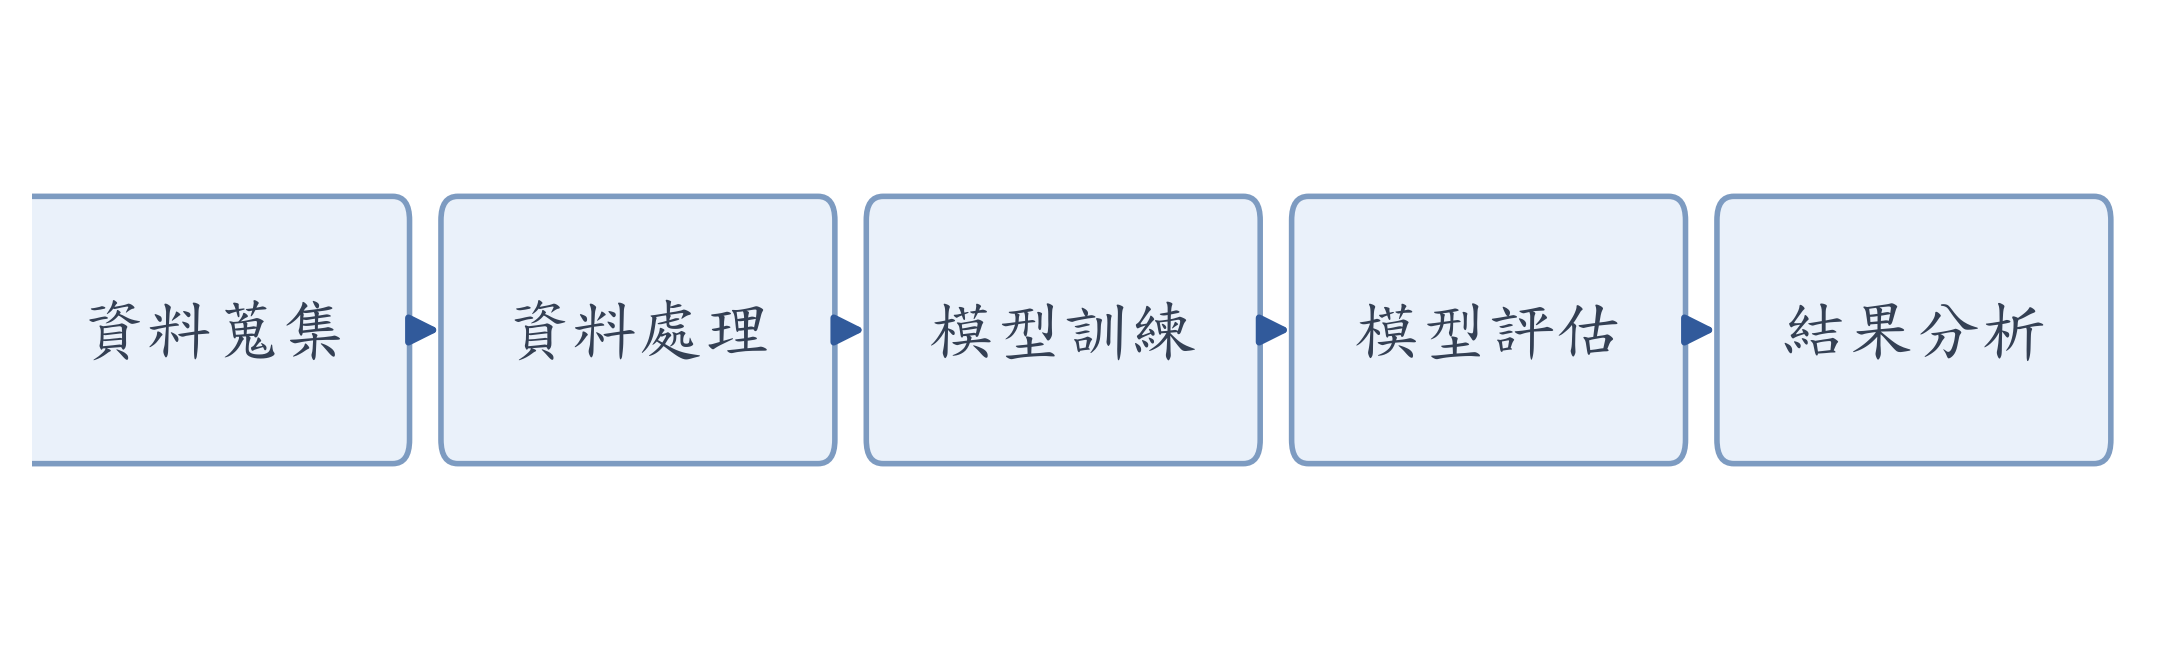
\includegraphics[width=0.6\linewidth]{figures/samples/architecture.png}
  \caption{說明}\label{fig:special}
\end{figure}
\end{lstlisting}

若想讓某一張圖只顯示編號、不顯示前綴文字，可以用 \code{\caption*} 不編號，或自行調整 \code{caption} 套件的 \code{\captionsetup}，詳見 \href{https://ctan.org/pkg/caption}{caption 的文件}。

\section{註腳}

圖表若需要額外補充，前面的分組表頭範例是在儲存格加上 \code{\textsuperscript{a}}，再對應 \code{notes} 裡的說明；但那只是手刻的上標文字，不是真正的註腳。若要在內文中隨插隨用、由 \LaTeX{} 自動編號與排版的註腳，可以改用 \code{\footnote{...}}，不需要另外編輯任何檔案，編號、上標與頁尾的分隔線都是自動處理：

\begin{lstlisting}[language=latex]
這一點有些爭議\footnote{不同研究對此看法不一。}，後續章節會再討論。
\end{lstlisting}

編譯後如下：

這一點有些爭議\footnote{不同研究對此看法不一。}，後續章節會再討論。

當頁最下方，編號從 1 開始，全文連續累加，不會因為換頁而重置。若同一個註解要在多處引用，先幫第一次出現的 \code{\footnote} 加上標籤，之後就能用 \code{\footref} 重複使用同一個編號，不會另外產生新註腳：

\begin{lstlisting}[language=latex]
第一次提到\footnote{說明文字。}\label{fn:first}，第二次提到時\footref{fn:first}。
\end{lstlisting}

編號格式與是否每章重新編號，都在 \code{config.yml} 的 \code{layout:} 下設定：

\begin{lstlisting}[language=yaml]
layout:
  footnote-numbering: "1"      # 1 | a | A | i | I | *
  footnote-per-chapter: false  # true 讓每章從 1 重新編號
\end{lstlisting}

\code{footnote-numbering} 的寫法跟 \code{outline.body-numbering} 等編號設定一樣，\code{"1"} 是阿拉伯數字，\code{"a"}／\code{"A"} 是英文字母，\code{"i"}／\code{"I"} 是小寫／大寫羅馬數字，\code{"*"} 則是星號、雙星號依序遞增，適合整篇註腳不多的論文。\code{footnote-per-chapter} 預設 \code{false}，註腳編號連續累加到全文結束；系所若要求每章重新從 1 編號，改成 \code{true} 即可，不需要自己在每章開頭手動歸零。

圖表、註腳與公式的寫法確認後，下一章會接著說明文獻引用，以及程式碼與附錄的寫法。
